%% File: elsarticle.latex
%% Purpose: Support Elsevier's `elsarticle` package through pandocomatic.
%%          To that end turn the generic `elsarticle-template.tex` into
%%          a template that can be used in conjunction with
%%          pandocomatic and scrivomatic.
%% Authors: Ian Max Andolina, Paul Brandt
%% Date   : Nov. 11, 2021
%% 
%% This file is a manual integration of:
%%      *   elsarticle-template.tex (NOT the `elsarticle-template-*.tex` 
%%          examples that appear in the elsarticle template for these are  
%%          not comprehensive enough for a full article).
%%          Sourced from https://www.latextemplates.com/template/elsarticle-academic-journal
%%      * custom.latex, a minimal portion of it to make it compatible with 
%%          pandocomatic, and removing those parts that potentially 
%%          redefine `elsarticle` definitions.
%%          Sourced from https://github.com/iandol/dotpandoc/tree/master/templates
%%
%% Backwards compatibility with both files need to be managed manually.
%%  
%% Usage notes:
%%      1 - You'd want to apply this in combination with:
%%          * pandocomatic-elsarticle.yaml, or its contents integrated
%%              in any other pandocomatic.yaml file
%%          * (optional) addstyles.sty
%%      2 - Connect <your>.md with pandocomatic's `elsevier` template
%%          * just like any other regular pandocomatic template, hence
%%          * Insert in <your>.md's yaml block:
%%            pandocomatic_:
%%              use-template:  
%%                - elsevier  
%%      2 - Run pandocomatic with <your>.md text as follows:
%%          * pandocomatic -b -c ./pandocomatic-elsarticle.yaml ./<your>.md
%%            This will generate <your>.tex, hence continue with
%%          * latexmk -interaction=nonstopmode -f -pv -time -xelatex <your>.tex
%%            This will generate <your>.pdf
%%            
%%
%% Regarding elsarticle ::
%% ---------------------------------------------
%%
%% Copyright 2007-2020 Elsevier Ltd
%% 
%% It may be distributed under the conditions of the LaTeX Project Public
%% License, either version 1.2 of this license or (at your option) any
%% later version.  The latest version of this license is in
%%    http://www.latex-project.org/lppl.txt
%% and version 1.2 or later is part of all distributions of LaTeX
%% version 1999/12/01 or later.
%%  
%%
%% Regarding dotpandoc's custom.latex ::
%% ---------------------------------------------
%% The template custom.latex is a fairly complicated piece of work 
%% (thanks to Ian Max Andolina) to produce scientific articles in a simple
%% workflow with Scrivener, pandocomatic and scrivomatic. 
%% I've taken bits and pieces from it to make the elsarticle-template
%% produce a tex document by application of a pandocomatic.yaml configuration.
%% 
%% 
%%%%%%%%%%%%%

\documentclass[sort&compress,preprint,authoryear,3p,twocolumn]{elsarticle}
%%
%% !Todo!: Resolve the conflicting `&` in `sort&compress` when parameterized as
%%         `classoption` in pandocomatic-elsarticle.yaml configuration.
%%         Currently, this parameter is added here directly as opposed to
%%         being pandocomatically configured.
%% !Todo!: Check whether one- or two-column mode has been selected, and
%%         establish the need to redefine Figures/Tables as done below.

%%%%%%%%%%%%% REQUIRED PACKAGES
%% The following packages are required for this template to remain compatible 
%% (or at least effective) with the Elsevier template.

%% Supporting colored links in citations to the References section.
\usepackage{xcolor}

%% The amssymb package provides various useful mathematical symbols
%% whereas the amsthm package provides extended theorem environments
\usepackage{amsmath,amssymb}

%% The hyperref package is required since pandocmatic inserts \hypertarget
%% around section titles and other inter-article linking.
\usepackage[]{hyperref}
% Setup hyperref to color the links, and insert authors, title and keywords
% as meta-data to the pdf document properties.
\hypersetup{
  pdftitle={Consolidating semantic interoperability in contemporary software architectural paradigms},
  pdfauthor={Paul Brandt, Eric Grandry, Marten van Sinderen, Twan
Basten},
  pdflang={en-GB},
  pdfkeywords={semantic interoperability, software
architectures, semantics, interoperability, design principles},
  colorlinks=true,
  pdfcreator={Scrivomatic, Pandoc and LaTeX}
}
%%

%%
%% Elsevier bibliography styles
%% ----------------------------
%% 
%\usepackage[authoryear]{natbib}
\bibliographystyle{elsarticle-harv}
%\setcitestyle{authoryear,open={(},close={)}} %Citation-related commands
%% Add extra options of natbib.sty, if any specified.

%%
%% !Todo!: Check the specifics of reference styles from elsarticle-template-*.tex
%%         as mentioned in https://support.stmdocs.in/wiki/index.php?title=Model-wise_bibliographic_style_files
%%         against the biboptions / bibliographicstyle settings from pandocomatic-elsarticle.yaml 
%% !ToDo!: Some of the bibliographicstyle settings require \usepackage{numcompress}. 
%%         Check whether this is included by this very template.
%%

%% 
%% Handle figures and tables in two-column mode
%% --------------------------------------------
%% In a two-column paper, figures and tables can become too small or overflow
%% the column width. In two-column mode we need to restore the original 
%% behaviour:
%% - For figures and tables, one needs to use the starred version * of these 
%%   environments. This floats the environment to the top/bottom of page over
%%   both columns.
%%   Source: https://tex.stackexchange.com/questions/89462/page-wide-table-in-two-column-mode
%%   Hence, redefine those environments:
\makeatletter
\renewenvironment{figure}{%
  \begin{figure*}
 }{% 
  \end{figure*}
 }
\makeatother
\makeatletter
\renewenvironment{table}{%
  \begin{table*}
 }{% 
  \end{table*}
 }
\makeatother
%%
%% - Longtable & xltabular do not work well with multicolumns. Therefore, 
%%   redefine these environments to enforce a single column mode before
%%   its definition, and restore the two-column mode afterwards:
\usepackage{stackengine}    % !!See Note (1) at the bottom!! 
\usepackage{xltabular}		% Include longtable with column specifier X as in tabularx
\usepackage{booktabs}		% To enhance the quality of tables in LaTeX. 
                            % Guidelines are given as to what constitutes a 
                            % good table in this context.
\usepackage{etoolbox}       % Used for the \BeforeBegin- & \AfterEndEnvironment
\BeforeBeginEnvironment{longtable}{%
    \onecolumn%
}
\AfterEndEnvironment{longtable}{%
    \twocolumn%
}
\AtBeginEnvironment{longtable}{%
    \scriptsize%
}
\BeforeBeginEnvironment{xltabular}{%
    \onecolumn%
}
\AfterEndEnvironment{xltabular}{%
    \twocolumn%
}
%%   This is not an optimal solution since it can result in pages around the
%%   longtables that are partly blank unintentionally. Other solutions to
%%   resolve this are welcome.
%%
%% !ToDo!: redefine simple tables, booktab and tabular.
%% !ToDo!: Make this part conditional on the documentclass-defined one- or
%%         two-column mode. That is, only include it when necessary.
%%

%%
%%%%%%%%%%%%% end REQUIRED PACKAGES

%%%%%%%%%%%%% OPTIONAL PACKAGES
%% The following packages are optional for this template, as
%% per the Elsevier template .

%% For including figures, graphicx.sty has been loaded in
%% elsarticle.cls. If you prefer to use the old commands
%% please give \usepackage{epsfig}

%% The lineno packages adds line numbers. Start line numbering with
%% \begin{linenumbers}, end it with \end{linenumbers}. Or switch it on
%% for the whole article with \linenumbers.
\usepackage{lineno}
\modulolinenumbers[5]

%% When you have an Orcid ID (refer to) you might want to include that
%% in your author-field as \orcidlink{<orcid>}
\usepackage{orcidlink}

\usepackage{blindtext}

%%
%% Some pandocomatic-specified options require additional packages
%%


%% Tightlist
\setlength{\emergencystretch}{3em} % prevent overfull lines
\providecommand{\tightlist}{%
  \setlength{\itemsep}{0pt}\setlength{\parskip}{0pt}}
%%

%%
%%%%%%%%%%%%% end OPTIONAL PACKAGES

%%%%%%%%%%%%% PROJECT SPECIFIC PACKAGES 
%%
%% These are managed through the `include-in-header:` parameter in the 
%% pandocomatic.yaml specification. Directly by listing the packages there, or 
%% indirectly by specifying one single file, e.g., `addstyles.sty`, that 
%% collects the required packages.
%% File   : addstyles.sty
%% Purpose: To include project specific packages without the need to insert
%%          multiplpe `header-includes:` statements in the 
%%          pandocomatic.yaml configuration file. 
%%          Although there is no functional difference between both approaches,
%%          for me this file seems to provide me with a more simple overview
%%          about which packages and their whereabouts. 
%%          Note that for this approach to work, you need to insert the name
%%          of this file in the `header-includes:` statement.     
%% Author : Paul Brandt, date Nov. 11, 2021
%%%%%%%%%%%
%
% Add your .sty files below
%
%   One can make a differentiation in where to store specific addons to your
%   LaTeX environment:
%   - Generics, i.e., re-usable ones, are maintained in folders below your TeX  
%     home directory. Use `kpsewhich -var-value=TEXMFHOME` at the command prompt 
%     to find your TeX Home. But respect the TeX Directory Structure (TDS) from
%     TeX Home downwards.
%   - Project specific stuff can be maintained in the same folder as your 
%     document for this project. 
%   No particular assumptions are made by the elsarticle templates with regard to 
%   locations of files.
%
%%%%%%%%%%%

\usepackage{mySemantics}
\usepackage{cleveref}		% sourced from http://tug.ctan.org/macros/latex/contrib/cleveref/cleveref.pdf 
                            % Makes varioref clever, and reuses its work to improve its own workings. 
							% The cleveref package must be loaded after all other packages that 
                            % don’t specifically support it. Therefore, to be safe, we declare it as last 
                            % in the document's preamble.
							% Also note that all \newtheorem definitions must be placed after the 
                            % cleveref package is loaded.
\usepackage{myTheorems}
\usepackage{myTables}

\usepackage{pdflscape}      % Extends package <lscape> to add PDF support to the environment `landscape`.  
                            % Applied for table on design Principles

\usepackage{afterpage}      % Causes the commands specified in its argument to be expanded after the current 
                            % page is output. The current page will be filled up with text after \afterpage{...}.
                            % Applied for table on design Principles

\usepackage{graphicx}       % Optimizes \rotatebox 
                            % Applied for table on design Principles

\usepackage{enumitem}		% List manipulation. Customize the three basic list environments 
                            % (enumerate, itemize and description) and design your own lists, 
                            % with a〈key〉=〈value〉syntax.
                            % Applied for table on design Principles

\usepackage{gensymb}        % The gensymb package provides a number of ‘generic’ macros, 
                            % which produce the same output in text and math mode. 
                            % Used for \celsius
                            
%%%%%%%%%%%
%% End of File: addstyles.sty
%%%%%%%%%%%

%%
%%%%%%%%%%%%% end PROJECT SPECIFIC PACKAGES

%%%%%%%%%%%%% DEPENDENCIES
%% When including packages by header-includes, 
%% dependencies might occur with them.
%% Resolve these dependencies below this line.
%%

%% Dependent on package{graphicx}
% Scale images - calculate the maximum dimensions first
\makeatletter
\def\maxwidth{\ifdim\Gin@nat@width>\linewidth\linewidth\else\Gin@nat@width\fi}
\def\maxheight{\ifdim\Gin@nat@height>\textheight\textheight\else\Gin@nat@height\fi}
\makeatother
% Scale images if necessary, so that they will not overflow the page
% margins by default, and it is still possible to overwrite the defaults
% using explicit options in \includegraphics[width, height, ...]{}
\setkeys{Gin}{width=\maxwidth,height=\maxheight,keepaspectratio}
% Set default figure placement to htbp
\makeatletter
\def\fps@figure{htbp}
\makeatother
%%

%%
%%%%%%%%%%%%% end DEPENDENCIES

%%%%%%%%%%%%% ADD & PARAMETERIZE elsarticle template elements

\journal{Information and Software Technology}

\begin{document}

\begin{frontmatter}

%% TITLE elements
  \title{Consolidating semantic interoperability in contemporary
software architectural paradigms\tnoteref{id1}}
  \tnotetext[id1]{version 2.0-0}
%%

%% AUTHOR elements
\author[1]{Paul
Brandt\fnref{0000-0002-2353-967X}\corref{corrauth}}\fntext[0000-0002-2353-967X]{ORCID: \orcidlink{0000-0002-2353-967X}0000-0002-2353-967X}\ead{paul@brandt.name}\cortext[corrauth]{Corresponding author} \author[2]{Eric
Grandry}\ead{egrandry@gmail.com} \author[3]{Marten van
Sinderen}\ead{m.j.vansinderen@utwente.nl} \author[1]{Twan
Basten}\ead{a.a.basten@tue.nl}
%%

%% INSTITUTE elements
\affiliation[1]{organization={Eindhoven University of Technology (TU/e),
Eindhoven, The Netherlands}} \affiliation[2]{organization={Ministry of
Mobility and Public Works, Luxembourg,
Luxembourg}} \affiliation[3]{organization={University of Twente (UT),
Enschede, The Netherlands}} 
%%

%% ABSTRACT text
\begin{abstract}
\emph{Background:} In today's increase of business digitalisation and
system's distribution, absence of access-and-play semantic
interoperability (sIOP) is a major hurdle to IT-based business
collaboration. Current approaches towards sIOP still rely on conventions
on the semantics of the exchanged terms, which can be considered both
accepted folklore and an impediment to access-and-play sIOP. A
breakthrough for this impasse requires consensus on the foundations of
semantics and sIOP. In a previous paper we already conclude that in
software, semantics cannot exist and is reduced to the reciprocity
between data and data processing code. We showed that semantics can be
addressed as separate concern, its reciprocity can be contained and
become a tangible artifact from which semantic reusability and
interoperability emerge as engineering benefits. For sIOP to emerge, the
effort of the inevitable human-in-the-loop is to be reduced and her
position improved. This is a matter of software architecture.

\emph{Objective:} The objective of our study is to identify and
formulate the fundamental demands towards access-and-play
interoperability, to derive their supporting architectural principles,
and their integration in contemporary architectural paradigms.

\emph{Method:} We follow a design-science approach and address the
business relevance of the problem, and identify six requirements on
sIOP, two of which are concerned with a genuine understanding of
semantics that demand for the human-in-the-loop. We assume that the
collaborating agents have followed the architectural principles on
semantics according to our previous study, which results in an explicit
representation of an atomic semantic monolith for each of the agents:
two semantic anchorages. We subsequently develop four design principles
in order to support interoperability between the semantic anchorages,
and one design principle to cater for the semantic distinction between a
formal semantic correspondence and the necessary data transcription
during communication. We finally evaluate these principles by designing
and formulating an ISO-42010 Architecture Viewpoint and View on sIOP.

\emph{Results:} Semantics in software are the result of a reciprocity
between data and the software code that operates on them, resulting in a
local semantic monolith \citep{Brandt2018a}. Data exchange breaks that
semantic monolith and hence the aforementioned reciprocity. The main
concern of sIOP is to re-establish a valid reciprocity between the
internal data processing code from the receiving agent and the external
data as received from the producing agent, without extending the
semantic monolith from either agents. We show that loosely coupled
semantics, semantic alignments and a shared ontological commitment of
the applied modelling language can be considered the cornerstone to
achieve sIOP. The supporting principles are: (i) assume responsibility
for the semantics of one's data, (ii) maintain an explicit ontological
commitment, (iii) abstract semantics from the communication syntax, (iv)
align the internal and external semantic meaning of the exchanged data,
and (v) encapsulate how agents exchange semantic meaning. This results
in a loosely coupled semantics that is re-usable for every
interoperating peer agent, even those that are not anticipated for
during the agent's design. The resulting ISO-42010 Architecture
Viewpoint and View on sIOP, including a semantic mediation capability,
represents a pattern to consolidate sIOP in contemporary architectural
paradigms.

\emph{Conclusions:} The major shortcomings in architectural paradigms to
account for an access-and-play sIOP are their negligence of a separation
of concerns between the semantic representation and data communication
syntax at the one hand and human-authored alignments and the automated
mediation process at the other, and establishing the conditions for
their support in advance. By their explicit inclusion, we show that
loosely coupled semantics can be consolidated in contemporary
architectural paradigms, stimulating access-and-play sIOP.
\end{abstract}

%%Graphical abstract
%\begin{graphicalabstract}
%\includegraphics{grabs}
%\end{graphicalabstract}

%%Research highlights
%\begin{highlights}
%\item Research highlight 1
%\item Research highlight 2
%\end{highlights}
%%

%% KEYWORDS elements
\begin{keyword}
semantic interoperability\sep software
architectures\sep semantics\sep interoperability\sep design principles
\end{keyword}
%%

\end{frontmatter}

%% Consider the use of line numbers
\linenumbers


%%%%%%%%%%%%% MAIN TEXT

\hypertarget{introduction}{%
\section{Introduction}\label{introduction}}

Never before, data were so ubiquitous, and managed access to external
data was so easy. But \emph{understanding precedes use}, and
understanding the data requires a human-in-the-loop and, therefore, is
time-consuming and hampers agility in business collaboration in all
domains. For instance, consider the following (allegedly real) example
of an interoperability failure.

\begin{quote}
A German steel producer upgraded its industrial process robot. Since the
majority of the steel production process is dependent on time, from a
safety point of view the decision was made to not rely on their own
internal clocks but to use the German \emph{Braunschweig Funkuhr} time
radio signal as source for the exact time instead. At the end of April
1993, when Germany went on summer time, the computer clock of the steel
producer went from 1:59 AM to 3:00 AM in one minute. This resulted in a
production line allowing molten ingots to cool for one hour less than
normal. When the process controller thought the cooling time had
expired, its actions splattered still-molten steel, damaging part of the
facility.\footnote{Source: http://catless.ncl.ac.uk/Risks/14/57\#subj1,
  accessed May 20, 2018}
\end{quote}

In this simple example a tiny difference in the meaning of \texttt{time}
between the steel producer and the national time provider hampered
interoperability to the extend of damaging the steel facility. This tiny
difference rooted in the assumption by the steel producer that
\texttt{time} expressed a continuous scale whilst for the Braunschweig
Funkuhr, \texttt{time} denoted instant clock time for the yearly season
and therefore represented a non-continuous scale. In order to achieve
that both collaborators, here the Braunschweig Funkuhr and the steel
producer, can actually \emph{use} their peers data, the need exists to
design and implement wrappers that remove any inconsistency between the
variations that may occur in terms, structures, dimensions and what have
you. Many such variations exist, leading to a range of failures in
so-called \emph{semantic interoperability} (sIOP). Unfortunately, it is
fundamentally impossible to automate the production of wrappers, because
we need a genuine \emph{understanding} upfront, which computers still
cannot do. ``Despite the notoriously difficult philosophical questions
involved, semantic interoperability can be seen as an engineering
problem, namely that of effectively constraining interpretations towards
the ones that are considered allowable'' \citep[p.5, based on
\citet{Kuhn2009}]{Scheider:2012tj}.

The most disconcerting consequences of a lack of (automated) sIOP are
time-to-deliver, flat interoperability failures, and as seen above,
seemingly correct but quite invalid data analysis results leading to
faulty system behaviour. Current sIOP implementations are essentially
based on the (time-consuming) process of establishing a shared
convention on the semantics of the terms that are exchanged during
collaboration, requiring custom solutions and collaboration-dependent
software adaptations. Such conventions result in a semantic monolith,
which makes dealing with data that originated outside the monolith
impossible, unless again a time consuming (months) semantic adoption
process is applied. Moreover, these semantic conventions consider
semantic heterogeneity a bug instead of a feature necessary to achieve
semantic accuracy. Nevertheless, this conventions-based approach towards
sIOP is considered accepted folklore, even state of the art in ICT. In
view of the large uptake of the Internet, the Internet of Things (IoT),
cloud computing and big data, and in view of economical pressure to
intensify enterprise collaboration, we consider this approach ``too
little, too late''. Some form of automation is required to resolve these
issues, and we place formal semantics at its core.

The main objective of our work is to achieve sIOP as quickly as
possible, with as minimal effort as possible, for collaborations that
had not been foreseen and consequently could not be anticipated for
during design time of the (two or more) software agents.

In comparison, scalability was a big architectural concern in the past,
requiring custom solutions as well. In response to this concern,
scalability was standardised in the form of architectural patterns, and
finally totally embedded and hidden into the infrastructure. Similarly,
sIOP can be considered the architectural concern of this decade. We
first need to provide standardised solution patterns that address
semantic concerns before we can embed it in a technological
infrastructure. Only then we can claim that sIOP becomes transparent to
the developer, and only then we can take down the tight coupling between
semantics and the syntax of the shared data scheme. Where scalability
resulted in a huge increase in performance-demanding applications
against a fraction of the original costs and effort, business agility
will emerge once their semantics are accessible and semantic services
exist at the infrastructural level to adress them. Then sIOP becomes an
access-and-play operation that can be achieved in due time with data not
anticipated for during software design, and at any point in their life
cycle. Metaphorically speaking, we consider sIOP as a bridge overarching
a semantic gap: with \emph{anchorages} (local semantics according to
\citep{Brandt2018a}) on each side of the gap, with a \emph{spanning}
(semantic alignments) resting on them to structurally (semantically)
support the interoperability bridge, and with a \emph{roadway} (data
mediation) enabling the crossing of the (data) traffic. Finally,
architectural \emph{principles} provide the necessary guidance to the
architect for the various design decisions that effectively result in a
particular bridge over a particular (semantic) gap. This has been
depicted in \cref{fig:semantic-concerns}.

\begin{figure}
  \centering
  \begin{subfigure}[b]{.75\textwidth}
    \centering
    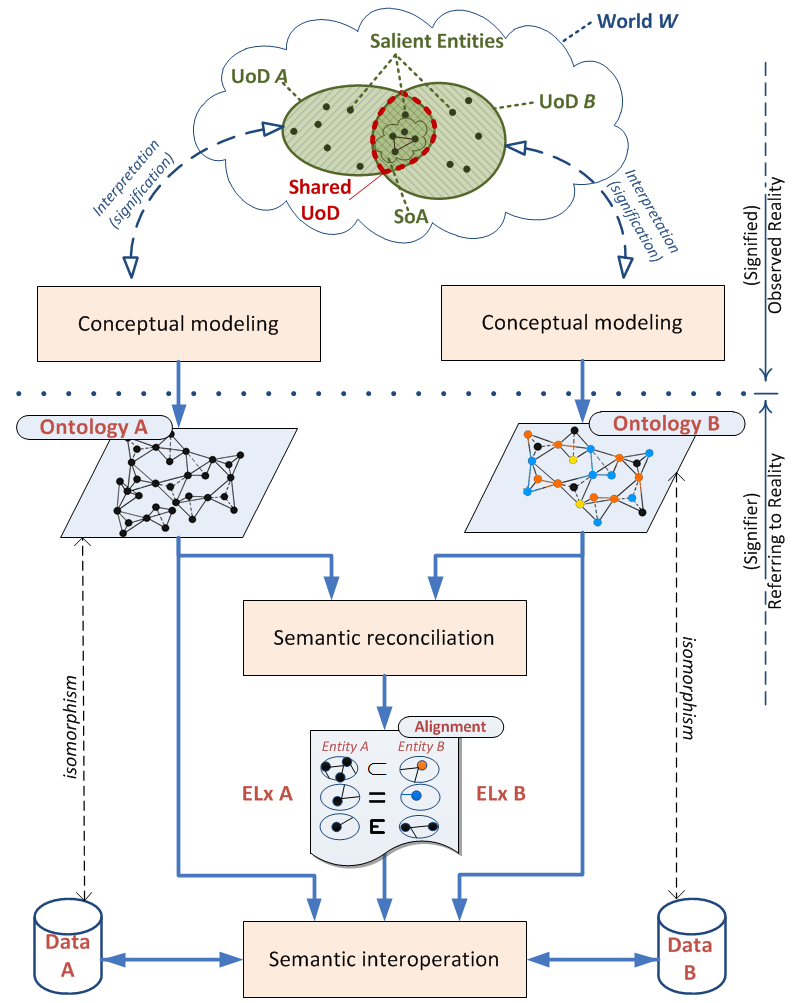
\includegraphics[width=\textwidth]{src/images/3SemanticConcerns.png}
    \caption{}
    \label{fig:concernsa}
  \end{subfigure}
  \hfill
  \begin{subfigure}[b]{.15\textwidth}
    \centering
    \includegraphics[width=\textwidth]{src/images/3ConcernsLegend.png}
    \caption{}
    \label{fig:concernsb}
  \end{subfigure}
  \caption{Conceptual overview of the relationships in sIOP between the anchorage (conceptual modelling), its spanning 
(semantic reconciliation) and roadway (semantic mediation), (a), and a legend explaining the used constructs (b).}
  \label{fig:semantic-concerns}
\end{figure}

Our contributions to consolidating semantic interoperability in software
architectures are fivefold, represented as architectural principles and
concerns as follows:

\begin{itemize}
\tightlist
\item
  Semantic concerns (anchorage): We summarize our work in
  \citep{Brandt2018a} on how to achieve a semantic anchorage by
  abstracting semantics from a tacit software implication into a
  tangible, computational and distinct artifact. This creates the
  potential to connect to it, to make comparisons with the semantic
  artifact of the peer software agent. We then formulate the principle
  of assuming responsibility on the semantics on data, and conclude what
  preparations about semantics are required for an agent before being
  able to engage in semantic interoperability
  (\cref{anchorage-semantic-concerns});
\item
  sIOP concerns (spanning): Since computers remain incapable of true
  understanding, sIOP remains in demand of human intervention in order
  to reconcile the semantic differences between collaborating software
  agents. However, human intervention is time consuming. We reduce the
  necessary human intervention to complement formal semantics to a task
  that suffices to achieve sIOP, viz.~authoring semantic alignments only
  (\cref{spanning-siop-concerns});
\item
  Mediation concerns (roadway): We determine the demands for a generic
  component that allows for communication with the peer agent in one's
  native vocabulary only, by considering both ontological models and the
  alignment. Such approach applies the principle \emph{connectivity
  without dependency} at the semantic level. This consolidates the
  agent's potential to collaborate to any unforeseen applications
  without the need to adopt external semantic definitions, and remain
  scalable in the process (\cref{roadway-mediation-concerns});
\item
  \emph{Evaluation of semantic principles}: In order to consistently
  address the above concerns, their founding architectural principles
  have been derived. It is a matter of architectural hygiene to evaluate
  how these principles support and consolidate the fundamental
  architectural demands about loose coupling and separation of concerns
  (notably semantics and communication concerns). We show how the
  necessary characteristics of semantics, i.e., semantic heterogeneity,
  semantic evolution and semantic scalability, are supplied by them
  (\cref{evaluation-of-siop-principles});
\item
  ISO42010 Architecture Viewpoint: We verify the applicability of the
  above concerns and principles by formulating their architectural
  consequences as a specific ISO42010 sIOP Viewpoint that must
  consolidate their proper position in the total architecture as
  corresponding sIOP view. As ISO42010 is considered a set of best
  practises for architecture description, and therefore is used with
  architecture frameworks such as MoDAF, TOGAF, DoDAF, RM-ODP and more,
  we conclude that application of this sIOP Viewpoint to formulate the
  sIOP View can be considered to consolidate sIOP for contemporary
  architectural paradigms (\cref{iso42010-viewpoint-on-siop}).
\end{itemize}

This could imply just another day in the office, because for ICT
architects and software engineers, refactoring the software agent in
order to separate distinct functionality into a new, valuable component
is one of their core skills. Application of architectural principles
bring about the new component, including an API and standard for its
access and use. Its adoption by IEEE, W3C, or a governing domain
organisation suffices for its integration at the right infrastructural
level. Quod non est for semantics, at least not that simple. ``The
successful standardisation of protocols made us believe that we should
also standardise meaning on the Web. This is a fundamental
misconception.'' \citep{Janowicz:2013ui}. Because, this is the first
time in the history of ICT that its discipline, viz.~we the ICT
community, are not speaking about a concern that belongs to the realm of
information and communication technology but to that of the users
instead. Consequently, we cannot control it, hence the existence of
semantic heterogeneity: how users represent what they mean and what is
meant with what is represented, differs between every so many
stakeholders. Despite this observation, current viewpoints on semantics
defy semantic heterogeneity and strive for semantic homogeneity: one
single agreed domain convention on how the syntactic representation and
structure of the data or messages shall be semantically interpreted.
Despite our, the ICT community, acceptance that semantics is a
representation of some part of the world, viewed from a particular
perspective of use, we don't acknowledge that this particular
representation and particular perspective is fundamental to the domain
users when building semantics and getting an understanding. And equally
important, we don't acknowledge that this particular perspective is just
one out of many equally legitimate ones that our software are deemed to
consider over the software's lifecycle. Some examples are given in
\cref{tab:perspectives}.

\begin{longtable}[]{@{}
  >{\raggedright\arraybackslash}p{(\columnwidth - 10\tabcolsep) * \real{0.2500}}
  >{\raggedright\arraybackslash}p{(\columnwidth - 10\tabcolsep) * \real{0.1724}}
  >{\raggedright\arraybackslash}p{(\columnwidth - 10\tabcolsep) * \real{0.1810}}
  >{\raggedright\arraybackslash}p{(\columnwidth - 10\tabcolsep) * \real{0.1810}}
  >{\centering\arraybackslash}p{(\columnwidth - 10\tabcolsep) * \real{0.0517}}
  >{\raggedright\arraybackslash}p{(\columnwidth - 10\tabcolsep) * \real{0.1638}}@{}}
\caption{Semantics follows many alternative but equally legitimate
points of view on reality, implying that no single one true
representation exists. Hence, semantic heterogeneity is a feature that
should be preserved, as opposed to a bug that should be sought to
correct. \label{tab:perspectives}}\tabularnewline
\toprule
\begin{minipage}[b]{\linewidth}\raggedright
Reality to refer to
\end{minipage} & \begin{minipage}[b]{\linewidth}\raggedright
Perspective \#1
\end{minipage} & \begin{minipage}[b]{\linewidth}\raggedright
Perspective \#2
\end{minipage} & \begin{minipage}[b]{\linewidth}\raggedright
Perspective \#3
\end{minipage} & \begin{minipage}[b]{\linewidth}\centering
\ldots{}
\end{minipage} & \begin{minipage}[b]{\linewidth}\raggedright
Perspective \#n
\end{minipage} \\
\midrule
\endfirsthead
\toprule
\begin{minipage}[b]{\linewidth}\raggedright
Reality to refer to
\end{minipage} & \begin{minipage}[b]{\linewidth}\raggedright
Perspective \#1
\end{minipage} & \begin{minipage}[b]{\linewidth}\raggedright
Perspective \#2
\end{minipage} & \begin{minipage}[b]{\linewidth}\raggedright
Perspective \#3
\end{minipage} & \begin{minipage}[b]{\linewidth}\centering
\ldots{}
\end{minipage} & \begin{minipage}[b]{\linewidth}\raggedright
Perspective \#n
\end{minipage} \\
\midrule
\endhead
Waves are & \emph{objects} that I can point at & \emph{forces} exerted
on dikes, walls or oil rigs & an \emph{accumulation} of other waves &
\ldots{} & a \emph{relation} between water, current, wind and the
seabed \\
\(\;\) & & & & & \\
How many terrorist attacks can be counted on 9/11? & 1, the number of
involved terrorist groups & 2, the number of collapsed towers & 4, the
number of involved aircraft & \ldots{} & 2996, the number of
casualties\footnote{as mentioned by Wikipedia,
  https://en.wikipedia.org/wiki/Casualties\_of\_the\_September\_11\_attacks,
  accessed Dec 13, 2018} \\
\bottomrule
\end{longtable}

We consider semantic homogeneity not only an illusion, but striving for
it brings about several important disadvantages. For instance,
implementation of semantic standards involves considerable expenses, and
tends to solidify in software by implicit operations on data. Moreover,
since semantic standards fix representation, semantics becomes conflated
with syntax, making the semantic standard dependent upon variations in
syntax and, hence, the architectural paradigm, its implementation or
applied technology. Together, this brings about a high impedance to
change or evolution, which creates a significant barrier for new
business opportunities, obstructing business agility. Finally, it is
sheer impossible to create for each particular domain, or part thereof,
a semantic standard; even in the highly protocolised health domain that
already addressed semantics in 1987 \citep{Spronk2014}, adoption of a
standard remains slow and cumbersome {[}REF{]}. This becomes all the
more clear when comparing with the successful adoption of 2G GSM
telecommunication standard, including its evolution to 2.5G, 3G, 3.5G,
4G and 5G standards during roughly the same era.

By separating syntactical from semantic concerns and turning semiotic
fundamentals into architectural principles, loosely coupled formal
semantics emerges and can be consolidated in contemporary architectural
paradigms. From that position embedding standard semantic services into
the communication infrastructure remains domain-independent; hence, for
us, the ICT-discipline, its standardisation can be considered yet
another day in the office again. We first describe some background on
the semantic foundations in the following section.

\hypertarget{anchorage-semantic-concerns}{%
\section{Anchorage: Semantic
concerns}\label{anchorage-semantic-concerns}}

It is clear that sIOP encompasses a communication between at least two
actors. And since we here talk about \emph{semantic} interoperability,
we consider the ability to explicitly connect the semantics from both
software agents a necessary condition for enabling sIOP. We defend that
software agents that might engage in interoperability should provide for
such semantic anchorage, i.e., taking responsibility over their own data
semantics, denoted the Domain Model in \citep{Brandt2018a}. In that same
paper we argued that such Domain Model should be represented in the form
of a domain ontology. Such ontology provides the ability for other
software agents to connect to the semantics of the subject agent in a
computational manner, consolidating the semantic concerns for semantic
interoperability.

It furthermore brings a natural responsibility for both actors in the
communication, described by \citep{Grice:1991BT} as the particular
purpose of communication, viz.~to serve:

\begin{enumerate}
\def\labelenumi{\arabic{enumi}.}
\tightlist
\item
  Quantity: Make your contributions as informative as is required (for
  the current purpose of the exchange), and not more than is required;
\item
  Quality: Do not say what you believe to be false, or for which you
  lack evidence;
\item
  Relation: Be relevant (to the immediate needs);
\item
  Manner: Avoid obscurity of expression, ambiguity, and be brief and
  orderly.
\end{enumerate}

Both aspects, explicitly connect the semantics of the interoperating
agents, and the need for each agent to take responsibility for achieving
the purpose the communication, represent the \emph{semantic concerns} of
sIOP. The maxim's Quantity and Manner immediately lead to the definition
of a design principle to their effect, and applying the normative
notation from \citep{Greefhorst2011} this reads as follows:

\begin{mmdp}[The responsibility for the semantic meaning of data lays with the source]\label{dp:rfsm}

When it is reasonable to expect that the software agent will be engaged in collaboration or otherwise will interoperate with (an)other software agent(s), it is the responsibility of the software architect to serve the quantity and manner of the potential interoperability by specifying the semantics of the data in advance. 

\textbf{Type of information:} business, data  \\
\textbf{Quality attributes:} semantics, interoperability, usability, efficiency   \\
\textbf{Rationale:}
\begin{enumerate}
  \item Data represent the state of affairs of some part of the world, viewed from a particular perspective of use. Such view is just one particular perspective out of many equally legitimate ones;
  \item Semantic heterogeneity, a direct consequence of the equally legitimate perspectives on reality, should not be considered a bug to resolve, but a feature to preserve and nurture in order to maximise semantic clarity and accuracy;
  \item Accepting semantic heterogeneity implies the probable uniqueness of the agents view on reality;
  \item Computers are not capable of genuine understanding, hence cannot establish semantics from data and thus require the human-in-the-loop for that;
  \item The responsibility for formulating the semantics that are expressed by the data can only lay by the software architect that has taken the particular perspective on reality when carving out the entities of interest to the software application;
  \item On specifying semantics, Grice’s maxims on communication, and particularly on serving the quantity and manner of communication, represent the natural constraints to respect;
  \item Without adherence to this principle, the meaning of the data expressed by the software agent can be considered flawed, inaccurate, incomplete or otherwise insufficient in its support for semantic interoperability.
\end{enumerate}
\textbf{Implications:}
\begin{enumerate}
  \item The specification of the data semantics is only dependent on the agent’s own perspective on the application domain, and can therefore be fulfilled before any specific interoperability with communication peers;
  \item No matter the number of different communication peers, the software agent needs to have the semantics of its data elements specified only once;
  \item By providing an explicit semantic specification of the data, an agent facilitates other components and agents to connect to it and, consequently, grounds its semantic interoperability with them unequivocally.
\end{enumerate}  
\end{mmdp}

Explicitly connecting the semantics of the interoperating agents
requires to firstly establish what is meant with semantics in software.
We argued in \citep{Brandt2018a} that since software is incapable of
genuine understanding, semantics cannot exist in software. Nevertheless,
the software agent acts as transport medium for semantics between users.
We further stated that the reciprocity between code and data does
manifest itself as software semantics. This essential disposition
discerns in semantics its \emph{semantic meaning}, i.e., what is said
and carried by data, and the \emph{pragmatic meaning}, i.e., to connect
with our frame of reference and its context of use, carried by code that
implements comprehension as an inference process from the semantic
meaning \citep{Grice:1991BT}. We explained that since data and code are
always tightly coupled and since their reciprocity emerges as software
behaviour, software malfunction originates (amongst others) from a
broken reciprocity, i.e., inconsistencies between data and code.
Consequently, when the data and code are representations of the things
and laws in the application domain and, hence, represents semantic
meaning and pragmatic meaning, their reciprocity represents the degree
with which the collective outcome of processing all potential data
faithfully refers to the intended states of affairs in reality. Any
incoherent reciprocity equates to unfaithfulness: semantics that are
considered invalid in the application domain.

Despite the quality with which the data and the code are developed
individually, we can maximise semantic validity by maximising their
reciprocity, viz.~demanding maximal coherence between code and data. We
have called this the \emph{semantic coherence principle}. The
consequence of this principle is the emergence of what we denoted the
\emph{Atomic Semantic Monolith} (ASM): being a semantic monolith refers
to the tight coupling of the reciprocity between data and their
processing code which, together, describe the state of affairs in the
application domain; Atomicity refers to the level of granularity at
which the entity that is referred to by the data token is considered a
non-dividable whole in the application domain. Where it is the objective
of semantics to maximise and maintain the coherence of the ASM, as
elaborated in (ibid.), it is the objective of sIOP to address this
monolithic nature of the ASM, as we do in the next section.

Where merriam-webster defines \emph{compatibility} as ``being a computer
designed to operate in the same manner and use the same software as
another computer''\footnote{Merriam-Webster,
  https://www.merriam-webster.com/dictionary/compatibility, accessed Jan
  2021}, we consider \emph{semantic compatibility} to reflect that an
actor is designed to interpretate according to the same semantic
principles and use the same ontological commitment as another actor. We
formulate the following design principle to its effect.

\begin{mmdp}[Semantic compatibility is a precursor to semantic interoperability.]\label{dp:eoc}

In order to consolidate semantic compatibility between collaborating agents, both agents must confess to their ontological commitment underlying their domain models.

\textbf{Type of information:} business, data  \\
\textbf{Quality attributes:} semantics, interoperability, usability, functionality   \\
\textbf{Rationale:}
\begin{enumerate}
  \item Semantic compatibility is a necessary condition for the emergence of sIOP;
  \item An ontological commitment represent a philosophical stance on fundamental categories and principles, which are foundational to semantics [@Brandt2021a, Sec.3.1];
  \item Each modelling language and, hence, every (domain) model, carries an ontological commitment, at least implicitly;
  \item The semantics of data as is specified by their domain model is subordinate to the categorisation and scope that follow from the ontological commitment of the applied modelling language; 
  \item Following [@Grice:1991BT], it testifies to the manner of communication to avoid obscurity of expression and ambiguity; 
  \item Without adherence to this principle, agents will suffer from semantic incompatibility and therefore experience significant issues with their capability to establish sIOP in their communication with each other.
\end{enumerate}
\textbf{Implications:}
\begin{enumerate}
  \item Actors that share the same ontological commitment will enjoy compatibility in the scope and nature of their semantics;
  \item Actors that don’t share the same ontological commitment will know to take corrective actions to assure their semantic compatibility;
  \item By providing an explicit specification of the ontological commitment underlying her domain model, an agent realises the proper semantic environment to establish semantic interoperability with her.
\end{enumerate}  
\end{mmdp}

\hypertarget{spanning-siop-concerns}{%
\section{Spanning: sIOP concerns}\label{spanning-siop-concerns}}

The semantic validity of any proposition can be assessed only if the
underlying ontological commitment can be referred to. Furthermore, any
assessment towards semantic interoperability of two semantic theories
cannot be made without an assessment of the similarity between their
underlying ontological commitments.

\hypertarget{objectives-of-semantic-interoperability}{%
\subsection{Objectives of semantic
interoperability}\label{objectives-of-semantic-interoperability}}

Semantic interoperability is about two software agents that share a
particular reality in their domains of application, and exchange data
that represent a certain state of affairs from that shared reality.
Despite the (different) reasons that both agents might have for sharing
the data, the only demand that is put on the exchange is to serve what
was coined by Grice as the communication's quality and relation: ``Do
not say what you believe to be false, or for which you lack evidence''
and ``Be relevant to the immediate needs''. Subsequent to the exchange
the data will be processed by the receiving agent and it stands to
reason that understanding the data precedes their faithful use. In
conclusion, semantic interoperability discloses the capability between
two software agents to use exchanged data that faithfully represent the
state of affairs that are relevant to consider about the shared reality
at that moment.

We have seen that software semantics is necessarily reduced to the
reciprocity that exists between data and their processing code in the
atomic semantic monolith, and that the ASM has been established with the
explicit purpose to guarantee the coherence between the data and their
processing code. Unfortunately, by exchanging data this data are
necessarily separated from the ASM they belong to. (Why it is useless to
exchange the complete semantic monolith in order to establish sIOP, is
left as an exercises to the reader \footnote{Answer:
  \rotatebox{180}{Communicating the semantic monolith, although possible, results in a too narrow solution towards sIOP because this would require each agent to have an exactly equal perspective on reality, and to represent this in the exact same way. Although possible, this will rarely be the case.}}.)
The consequence of exchanging the semantic meaning (data) only,
therefore, is twofold: it loses its coherence with its original
pragmatic meaning (data processing code), and, the necessity for a new
reciprocity with the pragmatic meaning belonging to the receiving agent
emerges. Unless it can be guaranteed that this new emerging reciprocity
is as coherent as it needs to be, semantic interoperability cannot
emerge from the data exchange and phantom semantics will emerge in
stead. From this we conclude that the main task about establishing sIOP
is to re-establish coherence between the external semantic meaning and
the internal pragmatic meaning. Note that although they share the same
semantic meaning, the resulting semantic monolith of the receiving agent
allows to be different from the original semantic monolith. For example,
by exchanging a heartbeat both agents share the a semantic meaning about
the number of beats per second, however the pragmatic meaning can vary
between an indication of health for an health-care application or an
indication of performance potential in a sports application. Mutatis
mutandis, when the semantic meaning is represented differently between
both agents, the resulting semantic monolith from the receiving agent
can be semantically equivalent but syntactically quite different.

From this discussion we learn that the \textbf{prime objective} for sIOP
is to assure that the reciprocity between data and code remains truthful
to the state of affairs in reality. This relates for both the external
data and the data that can be inferred from them. The \textbf{second
objective} for sIOP to pursue is to ensure that the ASM's from both
agents remain independent from each other, viz.~establishing a
semantical loose coupling between both agents. Such loose coupling does
not require one single homogeneous view on reality, which aligns neatly
with the \textbf{third objective} for sIOP: to allow for semantic
heterogeneity. Distinct agents will probably maintain alternative but
equally legitimate points of view on reality, implying that semantic
heterogeneity is a feature to preserve \emph{necessarily}. The
\textbf{fourth objective} of sIOP is to strive for access-and-play sIOP:
ideally, sIOP between agents can be achieved instantaneously, also for
unforeseen collaborations. This objective is very hard to achieve
because when we accept that software is incapable of genuine
understanding, and when we accept that correct use of data is to be
preceded by its understanding, a human-in-the-loop to provide that
understanding becomes a necessary condition for sIOP. The \textbf{fifth
objective} of sIOP is to allow for semantic evolution and, consequently,
the maintainability of sIOP. Finally, we consider that semantic
heterogeneity brings about an issue of scalability, since semantics
won't be centrally coordinated anymore; in stead, semantic definitions
will be distributed all over the place. We therefore include as
\textbf{sixth objective} of sIOP to allow for scalable semantics.

We conclude that from these six objectives, only the first (re-establish
reciprocity) and fourth (access-and-play) are concerned with genuine
understanding of semantics which demands for a human-in-the-loop. The
others are equally important in order to achieve sIOP, however, ``only''
refer to engineering challenges. We firstly address the first and fourth
objectives.

\hypertarget{positioning-the-human-in-the-loop}{%
\subsection{Positioning the
human-in-the-loop}\label{positioning-the-human-in-the-loop}}

We maintain the position that computers lack the capability for genuine
understanding and, hence, need to position the human-in-the-loop as a
necessary element in sIOP in order to cater for the understanding of the
semantic differences between the interoperating agents. This human is
required for one task only: re-establishing reciprocity. The two
possible approaches for this task are, (i) to modify the own pragmatic
meaning such that it can operate in a valid way on the external semantic
meaning, or (ii) to modify the external semantic meaning such that it
can be operated on by the existing pragmatic meaning in a manner
faithful to the current state of affairs. The consequence of the first
approach is that it allows external definitions to influence internal
workings. This clearly breaks one of the fundamental principles of
software engineering, \emph{low coupling, high cohesion}
\citep[e.g.,][]{Hitz1995}, and should therefore only be considered as a
last resort. The second approach only adapts that what was already
external to the receiving software agent, and thereby doesn't breach
this fundamental principle. We elaborate on this approach from the
perspective of the receiving agent. The task is to convert the
representation of the external semantic meaning such that it becomes
syntactically identical to the representation of the internal semantic
meaning, \emph{and}, that the original external ASM refers to a state of
affairs that is also referred to by the state of affairs of the internal
ASM when processing the external data.

In order to achieve that, we first assume that the quality of our own
software agent is such that the internal semantic meaning is in
coherence with the internal pragmatic meaning, i.e., that its concerning
ASM is faithful to reality over the complete range of the internal
semantic meaning, i.e., the data values that it is designed to process.
Contrarily, we \emph{cannot} assume that any variation on the internal
semantic meaning, no matter how small, will remain in coherence with the
internal pragmatic meaning. Founded on this essential disposition we
conclude that aligning the external semantic meaning with the internal
semantic meaning such that the former does not overlap the latter, is
the only approach that can guarantee sIOP. We reflect this with the
following principle:

\begin{mmdp}[Align the internal and external semantic meaning of the exchanged data]\label{dp:alignment}

When a software agent engages in interoperation with (an)other software agent(s), establish for the exchanged data a maximal coherence between external semantic meaning and internal pragmatic meaning by formalising the alignment between the external and internal semantic meaning.   

\textbf{Type of information:} application, data  \\
\textbf{Quality attributes:} semantics, semantic interoperability   \\
\textbf{Rationale:}
\begin{enumerate}
  \item On processing external data, semantics manifest themselves as the reciprocity between data and processing code;
  \item Data are considered to carry the semantic meaning as specified by the Domain Model of the software agent;
  \item Formalising a correspondence relation between the semantic meanings of interoperating software agents effectively connects the external semantic meaning with the internal pragmatic meaning;
  \item By assuring that the internal semantic meaning encompasses the external semantic meaning, and by assuring that the semantic consequences of the latter extending the former are insignificant, collectively assures the semantic validity of the correspondence relation.
\end{enumerate}
\textbf{Implications:}
\begin{enumerate}
  \item The conversion from external to internal semantic meaning is specified by a correspondence;
  \item The collection of all correspondences specify the semantic alignment that holds between a pair of interoperating agents;
  \item Software agents that are unable to align their semantic meaning with the external semantic meaning cannot engage in sIOP without introducing phantom semantics, with unforeseen consequences in their data processing.
\end{enumerate}  
\end{mmdp}

A \emph{correspondence} specifies as accurately as possible the semantic
difference (out of those listed in Appendix A) that exists between a
pair of related concepts, i.e., it aligns between the semantic meanings
of interoperating agents. By exhaustively addressing all semantic
differences that exist between both agents, the set of correspondences
collectively specify the \emph{alignment} that holds between two agents.
The purpose of the alignment is to establish how the truth of
expressions that are formulated in terms of agent A, can be established
by using formulations in terms of agent A', and to capture their
potential difference as a relation. To that end we differentiate between
two categories of semantic differences:

\begin{enumerate}
\def\labelenumi{\arabic{enumi}.}
\tightlist
\item
  \emph{Conceptual differences}: variations that can be specified as
  logical relation between (constructions of) concepts from both
  ontologies, e.g., naming conventions or variations in structure;
\item
  \emph{Value differences}: variations in conventions on how to
  represent values with or without magnitudes, e.g., differences in
  value scales, units of measure or nominal properties.
\end{enumerate}

The language used to specify the correspondences must be expressive
enough to identify the atomic elements of the ontologies, to combine
them into logical combinations as well as to formulate the relationship
that holds between them. In \citep{Euzenat2007, Scharffe2011}, an
investigation has been reported towards the requirements for such an
alignment language, summarised as follows. A \emph{correspondence}
denotes a single particular inter-ontological relation, prescribed, and
assumed to represent a semantically valid relation between both
concepts, as: \begin{equation*}\label{eq:correspondence}
\mu = \tuple{ e, e’, \theta }
\end{equation*} with:

\begin{itemize}
\tightlist
\item
  \(\theta \in \set{=, \sqsubset, \sqsupset, \disj, \overlap }\)
  specifying the \emph{correspondence relation} that holds between
  entity constructions from the source, \(e\), and the target, \(e’\).
  The basic correspondence relations denote \(=\): semantic equivalence,
  \(\sqsubset\): subsumption of, \(\sqsupset\): subsumes, \(\disj\):
  disjointness, and \(\overlap\): overlap. Although more relations can
  be required to include for a particular use case, such does not
  invalidate the general principle. Further note the correspondence
  relation is a directed relationship.
\item
  The source and target \emph{entity constructions}, \(e\), are build on
  the atomic elements of the ontology language. An entity construction
  connects concepts by applying:

  \begin{itemize}
  \tightlist
  \item
    conceptual connectors:

    \begin{itemize}
    \tightlist
    \item
      logical connectors \token{AND}, \token{OR}, and \token{NOT};
    \item
      a path connector as a sequence of zero or more Object Relations,
      \token{R}, optionally ending with an Object Property \token{P},
      summarised as follows: \token{R^*[P]};
    \item
      property construction operators (inverse, composition, reflexive,
      transitive and symmetric closures);
    \item
      constraints (through domain, range, cardinality and value
      restrictions);
    \end{itemize}
  \item
    value functions:

    \begin{itemize}
    \tightlist
    \item
      mathematical calculations for, e.g., unit conversion, operating on
      one or more values having a magnitude in order to arrive on a
      value that fits the dimension(s) of use by the pragmatic meaning
      of the receiving agent;
    \item
      transcriptors operating on one or more nominal values without
      magnitude, viz.~codes that identify or categorise a certain domain
      aspect, e.g., ISO3166-alpha2 two-letter codes that specify a
      particular country, or the blood type.
    \end{itemize}
  \end{itemize}
\end{itemize}

Without the conceptual connectors it is only possible to address a
single concept or individual as defined by the ontology, representing an
aggregation level that is relevant for the software agent but might not
be relevant in terms of the interoperating agent, and hence, for their
mutual sIOP. By application of conceptual connectors the architecture
gains the capability to address a specific compound of individuals in
either the source or target ontology that relate to the semantic
difference at hand. Similarly, with the application of value functions,
the architecture gains the capability to specify transformations between
conventions on value representations and nominal properties.

Current solutions that standardise semantic solidify the understanding
in the syntax of the data. In this way, semantics are carried by a data
schema that is primarily designed to serialise data and to support data
transfer by message construction and exchange. We consider this a
significant neglect of the principle on separation of concerns,
conflating the semantic interoperability concerns with the data
communication concerns. The consequence of conflating these concerns is
that source code which should concerned primarily with message
construction, parsing, storage, and other data communication related
tasks, becomes dependent on how semantics influence the syntax. In a
message-oriented paradigm, for instance, any difference in structure in
order to reflect the local perspective on semantic structure will have a
significant impact on how to (de)compose the message. And any new data
source to connect to will proliferate into a new software release. We
thus observe that the current approach to data understanding results in
an architecture which imposes a significant complication on
interoperability (and other -ilities as well), impeding access-and-play.
And despite the current limitations of AI-software to genuinely
understand, a significant gain towards the software agent's
access-and-play capabilities can be achieved by untangling the syntax
and semantics through separation of the sIOP concerns from the data
communication concerns. We propose the following design principle to its
effect:

\begin{mmdp}[Separate semantics from communication syntax]\label{dp:ssoc}

When a software agent engages in interoperation with (an)other software agent(s), resolve their semantic differences independently from the syntax of the exchanged data.   

\textbf{Type of information:} data, technology  \\
\textbf{Quality attributes:} semantic interoperability, portability, maintainability, efficiency, usability (reuse), reliability, functionality   \\
\textbf{Rationale:}
\begin{enumerate}
  \item Data schemata are defined to support the (de)serialisation processes that consolidate the data communications concern;
  \item Neglecting the principle of separation of concerns solidifies dependency between otherwise disjoint concerns, here the semantic level and the syntactic level of data communication;
  \item Access-and-play capabilities are supported by assuring minimal impact on software code when introducing semantic modifications;
  \item Minimising impact on software code that is concerned with data communication is realised by abstracting semantics away from the data schemata.
\end{enumerate}
\textbf{Implications:}
\begin{enumerate}
  \item Separation of concerns has a strong positive effect on software quality, including but not limited to sIOP;
  \item Removing any dependency between semantics and data syntax enables to support multiple communication paradigms without the need to modify the semantic abstraction;
  \item Similarly, modifications in the semantic representation, or supporting multiple semantic representations become possible without the need to modify the communication layer;
  \item Align semantics, not data schemata: Semantic reconciliation is applied at a higher conceptual level and abstracts away from data communication schemata;
  \item Heterogeneous semantics from multiple data sources are more easily supported;
  \item Semantic alignments imply the need for a mediation capability between the semantic representations of the communicating agents.
\end{enumerate}  
\end{mmdp}

Current sIOP practises already require humans-in-the-loop to reconcile
the semantic differences that occur. Often, the subject of
reconciliation is the differences in data schemata, and the result of
the reconciliation is laid down as a canonical data model. By applying
semantic reconciliation on the conceptual level, the dependency on the
(data) syntax, and vice-versa, is minimised. Moreover, by representing
the result of the reconciliation as an alignment (between ontologies) as
opposed to a canonical semantic model (core ontology), the influence of
the peer agent's semantics on one's own semantics is minimised as well.
An alignment, thus, functions as an interface that enforces loosely
coupled semantics by enabling semantic transparency between
communicating peers. Reducing the human-in-the-loop to author an
alignment only, (i) accelerates the deployment of sIOP by removing all
human effort that is concerned with implementation activities, and (ii)
decouples the sIOP scope to bilateral alignments only. This process has
been depicted in \cref{fig:dt-reconciliation}.

\begin{figure}
\hypertarget{fig:dt-reconciliation}{%
\centering
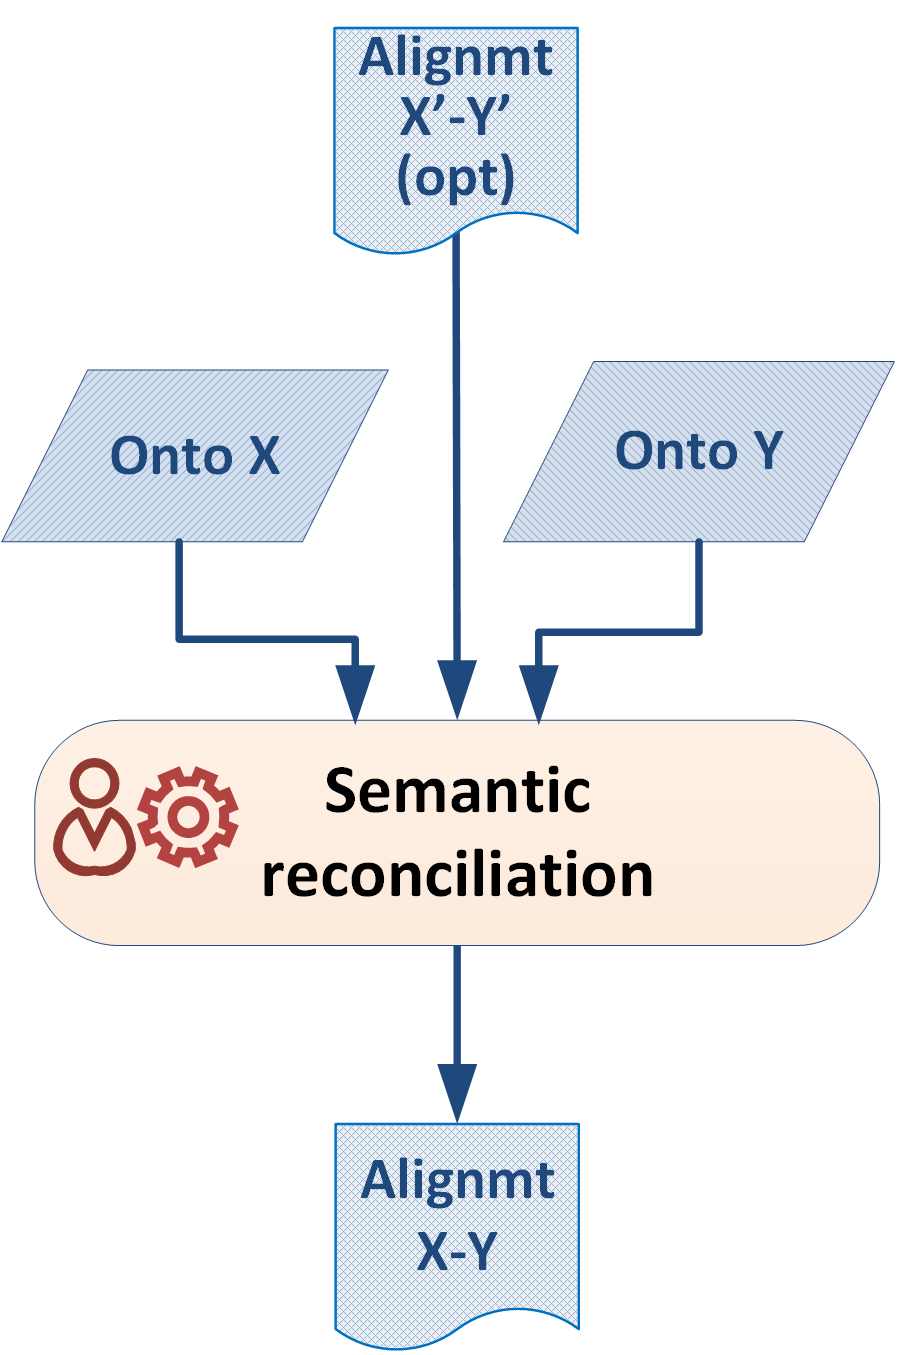
\includegraphics[width=0.25\textwidth,height=\textheight]{src/images/DesignTimeReconciliation.png}
\caption{Semantic reconciliation results in an alignment between the
semantic representations of two ontologies. We defend that semantic
reconciliation is a computer-aided but ultimately human-authored
task.}\label{fig:dt-reconciliation}
}
\end{figure}

\hypertarget{roadway-mediation-concerns}{%
\section{Roadway: Mediation concerns}\label{roadway-mediation-concerns}}

The mediation pattern has already been described in \citep{Gamma1994},
albeit in the context of object-orientation as opposed to sIOP. It is
described as ``an object that encapsulates how a set of objects
interact'', and it promotes loose coupling ``by keeping objects from
referring to each other explicitly'' and by enabling you to ``vary their
interaction independently''. In this way, the mediator turns a
many-to-many interaction into a many-to-one interaction, each of which
is easier to understand, maintain and evolve. The fundamental idea
behind the pattern, viz.~trading the complexity of the interactions with
the complexity in the mediator, can also be applied on a semantic level,
and we formulate the following principle to its effect:

\begin{mmdp}[Encapsulate how agents exchange semantic meaning]\label{dp:mediation}

When software agents engage in interoperation, encapsulate how the representation of their semantic meaning should be transcribed without inducing phantom semantics.   

\textbf{Type of information:} business, data  \\
\textbf{Quality attributes:} semantic interoperability   \\
\textbf{Rationale:}
\begin{enumerate}
  \item The semantic meaning is codified in (onto)logical representations;
  \item Keeping agents from referring to each others representation therefore requires transcription between representations;
  \item A solution where each agent needs to implement one transcription component between its own representation and each of its interoperating peer, increases complexity;
  \item Encapsulating the transcription into an alignment-based intermediary component results in less communication complexity and relieves the agents from development and maintenance of local wrappers;
\end{enumerate}
\textbf{Implications:}
\begin{enumerate}
  \item A mediator creates representational transparency between communicating agents, keeping agents from using each others representations;
  \item This enables independent development of the individual agent’s semantic meaning;
  \item The need to enforce a canonical semantic representation, viz. semantic homogeneity, expires, allowing semantic heterogeneity to become the norm;
  \item Each agent can reuse its semantic anchorage in any other interoperation;
  \item Data transcription logic can become a generic service provided by the communication infrastructure;
  \item Each agent can communicate with any other agent in its own native semantic representation.
\end{enumerate}  
\end{mmdp}

In this reading a mediator encapsulates how a pair of agents represent
their semantic meaning and provides for a generic transcription logic to
mediate between native semantic representations. However, one paramount
issue must be resolved by the transcription logic of the mediator, as
follows.

\begin{figure}
\hypertarget{fig:rt-mediation}{%
\centering
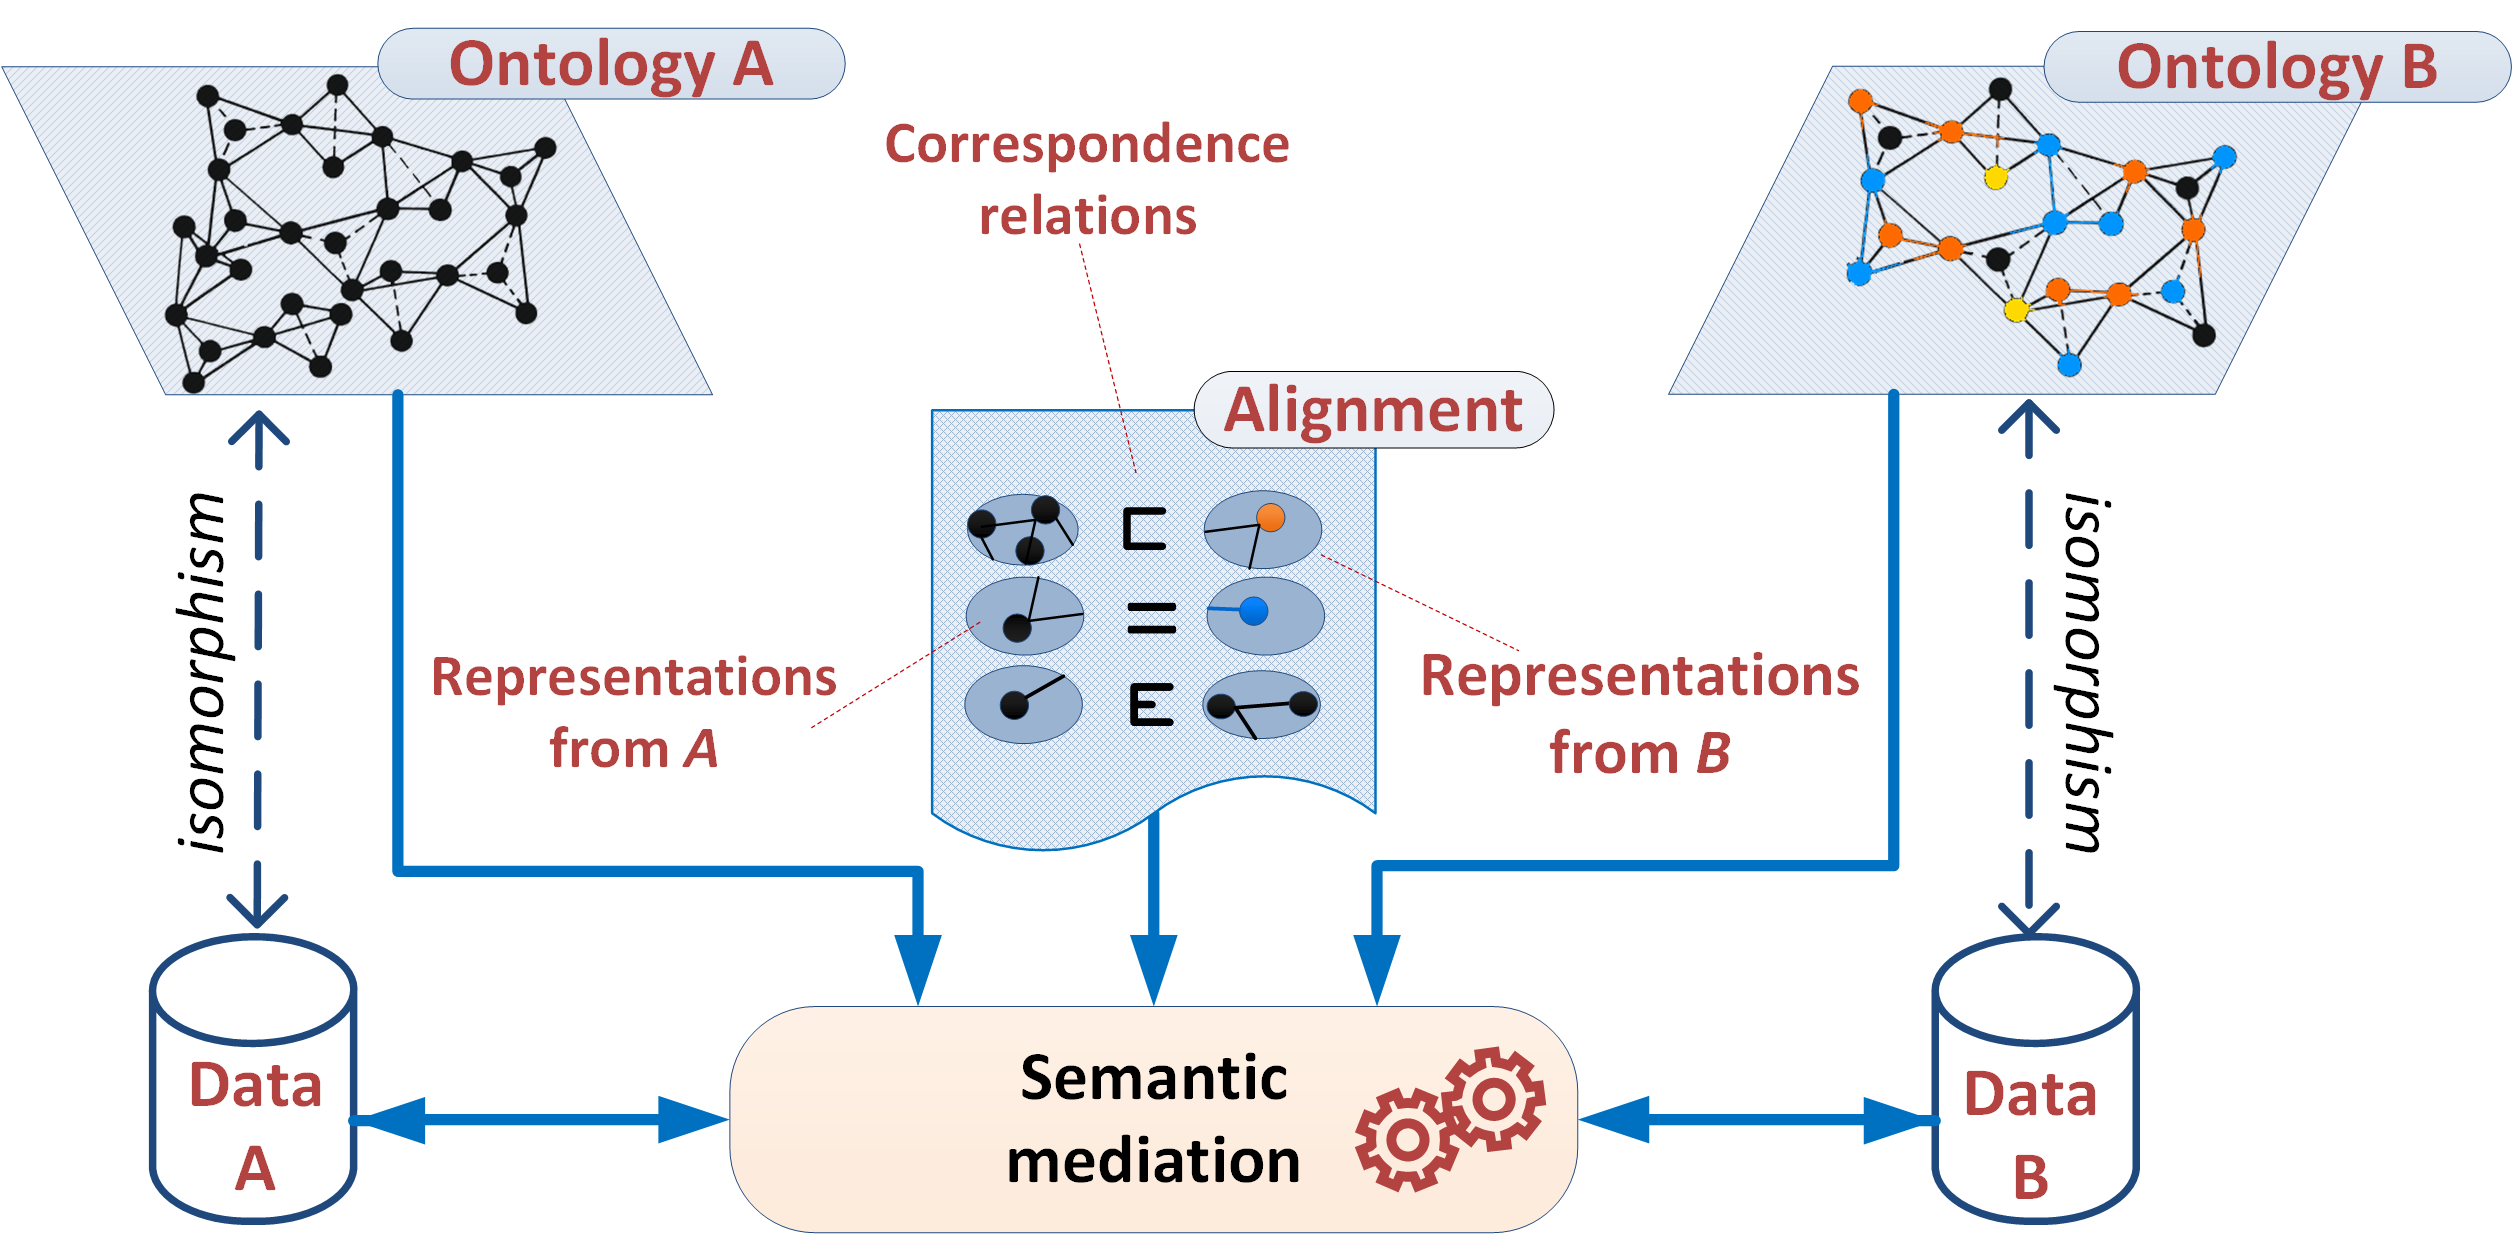
\includegraphics[width=0.75\textwidth,height=\textheight]{src/images/RunTimeMediation.png}
\caption{Semantic mediation encapsulates how agents exchange semantic
meaning. It implements a generic transcription service between the
particular representations of data between both agents. It depends only
on the representations of the semantic meaning from both agents
(ontologies) and the alignment that holds between
them.}\label{fig:rt-mediation}
}
\end{figure}

We have seen in the previous sections that a correspondence assures the
semantic validity between the different semantic meanings of both
agents. It can do so by token of the broad correspondence relations that
can be specified, both for the conceptual and the value differences that
may exist between them. Unfortunately, this is in shear contrast with
the fact that a transcription can only replace one term for another,
which basically implies that an equivalence relation holds between both
terms. As can be seen from the correspondence relation, this is not
necessarily true. In \citep{Brandt2018b}, we make a distinction between
a naive transcription, which ignores this inconsistency, and a semantic
valid transcription that can establish under what conditions this
inconsistency does not produce invalid semantics. We show that these
conditions rely on logical constructs only and, consequently, are
independent on the actual ontologies that apply. We have formulated
these logical constructs as rules that generically apply for any
transcription. Unfortunately, a set of conditions remain for which a
semantic valid transcription cannot be guaranteed, either due to an
incomplete alignment or to (onto)logical incorrect correspondences. It
follows that a semantic mediation service must provide for options about
the resolution for these remaining issues. We suggest at least the
following options: Firstly, as run-time options we consider (i) a means
to fall-back to the application of naive transcriptions and continue the
data exchange, or (ii) to raise a Transcription Error and refrain from
data exchange. Both represent necessary service implementations that
might satisfy scenarios that have either less or more stringent semantic
demands. Secondly, as design-time option, it serves as a necessary tool
to generate an exhaustive list of shortcomings of the transcription as a
result of the current ontologies and alignment. Such list will provide
the semantics engineer with sufficient information to adapt the
alignment, or introduce modifications to one or both of the semantic
anchorages in order to remove transcription issues that are considered
vital to the business. Finally, the third option is to try to resolve
the transcription issue by starting a dialogue-based semantic
reconciliation process in run-time with the aim to improve upon the
shortcomings of the current alignment. Despite our insistence on the
need for a human to author the genuine understanding, it might still be
worthwhile to have the system meticulously, consistently and
methodologically negotiate logical and ontological constructs in order
to find additional correspondences \citep{Diggelen:2007vd}.

\hypertarget{evaluation-of-siop-principles}{%
\section{Evaluation of sIOP
principles}\label{evaluation-of-siop-principles}}

The main (business) requirement is to achieve sIOP as quickly as
possible, with as minimal effort as possible, for collaborations that
had not been foreseen and consequently could not be anticipated for
during design time of the (two or more) software agents. We have
introduced some new principles to its support in the previous sections,
and now evaluate their consequences on objectives two (loose coupling at
semantic level), three (allow for semantic heterogeneity), five (support
to semantic evolution) and six (scalable semantics).

\hypertarget{loosely-coupled-semantics}{%
\subsection{Loosely coupled semantics}\label{loosely-coupled-semantics}}

Consolidating sIOP demands the emergence of \emph{loosely coupled
semantics}. As analogy, consider a vehicle with its cargo. Logistics
rely on external transfer services that allow the cargo to be
transported over different vehicles, from a truck into an aircraft into
ship into a truck again, without ruining the cargo. This requires the
cargo to be firmly connected to the vehicle, but at the same time to be
completely independent from any particular vehicle in order to complete
the transport. ``Connected but as independent as possible'', also known
as loosely coupled, is a need for sIOP as well. When software agents
interact they exchange meaning. Loosely coupled semantics implies that
the semantic meaning (the cargo) remains as independent from the
representation of semantics (the vehicle) as possible. Similarly to
logistics, sIOP should rely on infrastructural services that can
transcribe the semantic representation from its native form into a
foreign form without invalidating the semantics that it bears. Loose
coupling is known as a strong characteristic which brings many
advantages. This applies to its semantic variety as well: agents can now
communicate in their own native representations without the need to
learn or integrate foreign representations; define semantics once and
achieve sIOP many times with many different peers; development of the
agents' semantic representations can be locally isolated to fit their
particular domain and application; and it enables local re-use which on
its turn increases its quality.

Loose coupling in the classical sense is realised through the principles
of separation of concerns and transparency. In its original reading
separation of concerns turns complex functionalities into simple, atomic
and complementary functional capabilities. In a semantic reading
separation of concerns is not about maintaining complementary semantics;
in fact, the domain of interest of the agents are required to overlap,
since interoperation would be completely useless otherwise. Instead,
semantic separation of concerns refer to enforce an explicit division
between syntax and semantics, as discussed in
\cref{explicit-siop-by-alignment}. Additionally, it refers to keeping
each other's representations of the semantic meaning strictly separated.
We described how this can be achieved in \cref{roadway-mediation}. The
classical results of applying the principle is the emergence of unique
functions that are implemented only once and used many times. In its
semantic application this results in every software agent to maintain
its own semantics. Collectively, all agents make that semantics become
distributed all over the place which seems counterintuitive or even
plain wrong. We come back to that intuition when we talk about
scalability, \cref{scalable-siop}, but we can already see that this is
an indirect consequence of the demand to enable sIOP with agents that
were not anticipated for during software design; this, on its turn,
requires that independent development of semantics shall be possible
without disabling sIOP.

The classical reading on transparency separates access to the unique
functions from the particular design and implementation of the
functions. Remaining agnostic to \emph{how} its function are achieved
makes it possible to communicate with minimal mutual dependency.
Semantic transparency, or terminology transparency, remains agnostic to
how semantics are \emph{represented}, which makes it possible to
communicate with minimal syntactic dependency and without prior mutual
agreements on semantic representation. In its classical reading,
transparency requires the introduction of standards in the components'
API. Semantic transparency, contradictory, requires the total absence of
any standard on representation. In stead, semantic transparency, too,
requires to separate semantics from syntax. Furthermore, a need emerges
for a semantic oracle that knows how to align distinct representations
and to translate between them accordingly. The latter has already been
discussed in \cref{roadway-mediation} while the former is directly
related to the human-in-the-loop as authoring authority as discussed in
\cref{spanning-semantic-interoperability}.

From the above discussion we draw the conclusion that all demands
necessary to allow for semantic separation of concerns and semantic
transparency are met by the sIOP principles
\cref{dp:ssoc,dp:alignment,dp:mediation}. Therefore, loosely coupled
semantics should emerge between agents that comply to these principles.

\hypertarget{semantic-heterogeneity}{%
\subsection{Semantic heterogeneity}\label{semantic-heterogeneity}}

We have already determined that the principle to align semantics as
opposed to data schemata, \cref{dp:ssoc}, breaks the conflation of
semantics and syntax, enabling to consider semantics on its own
terms\footnote{Pun not intended}. Abstaining from a canonical model by
introducing a semantic alignment between pairs of semantic meanings,
\cref{dp:alignment} introduces the capability for each agent to develop
its semantic representation in a way that fits its local perspective
optimally. By also encapsulating the particular means to provide valid
semantic transcriptions only and refrain from naive transcriptions
between communicating agents, \cref{dp:mediation}, the necessary
elements to support semantic heterogeneity are present.

\hypertarget{semantic-evolution}{%
\subsection{Semantic evolution}\label{semantic-evolution}}

Consider an agent who's local semantics are in demand for a change.
Assume that the agent has modified its internal pragmatic meaning to
accommodate the evolved semantics. This implies a change in what we
called the semantic anchorage, which acts as semantic interface to any
sIOP concerns. The semantic change can be considered an altered or
additional difference with the semantic anchorage from interoperating
peer agents. In order to not destroy the sIOP that had been established
before, it is necessary to reflect the new difference as modifications
to the alignments that apply. By having performed the necessary
modifications, and by relying on the semantic validity of the own
ontology, the mediator is now capable of transcribing the data in
accordance to the evolved semantics.

The consequence of allowing semantic heterogeneity is therefore a
sufficient condition to also enable local semantic evolution and
remaining semantic interoperable with existing counterparts in the
process.

\hypertarget{scalable-siop}{%
\subsection{Scalable sIOP}\label{scalable-siop}}

Many definitions exist to constrain the semantics of \emph{scalability},
academic \citep[e.g.,][]{Neuman1994} and popular\footnote{http://www.linfo.org/scalable.html,
  accessed Nov.~2019; https://en.wikipedia.org/wiki/Scalability,
  accessed Nov.~2019} alike. Our summary refers to increasing the demand
that is placed on a system, and/or adding resources to a system, without
experiencing loss of performance or increase in management to an extent
that defeats its primary objective. We consider scalable sIOP as the
capability to allow for increase in number of communicating agents as
well as in the level of semantic heterogeneity without degrading the
agent's communication performance or its ability to manage and control
the semantic differences with its interoperating peers.

If we consider the agent's communicating performance degradation, we
argue that since complexity of the connections have been traded with the
complexity in the mediator (\cref{roadway-mediation}), the agent will
only experience communication degradation when the mediator experiences
transcription latencies that exceed communication parameters. In other
words, the performance bottleneck is with the mediator, not with the
agent. Transcription latency will result from the number of
transcription requests that exceeds the capacity of a single mediator.
No particular mechanism in a mediator impedes horizontal scaling to
increase the collective processing capacity to match the transcription
demands.

Regarding the ability to manage and control the semantic differences
with all interoperating peers, the root cause for potential alignment
management issues are laid in the need to establish an alignment with
each peer agent an agent collaborates with. This might become
impractical due to our insistence on the need for a human-in-the-loop to
author the alignment. We discern different solutions for different
semantic topologies:

\begin{enumerate}
\def\labelenumi{\roman{enumi}.}
\tightlist
\item
  Star alignments (core domain ontology, aligned to local ontologies)
  for relative stable and homogeneous domain semantics

  \begin{itemize}
  \tightlist
  \item
    Good: semantic governance remains controllable independent from the
    number of actors;
  \item
    Bad: very big semantic monolith, hence, low agility in dynamic
    environments. Moreover, the more actors involved, the higher the
    need for semantic compromises, and the lower the overall semantic
    accuracy.
  \end{itemize}
\item
  Mesh alignments (bilateral alignments) for very dynamic and
  heterogeneous (domain) semantics, or low number of peers

  \begin{itemize}
  \tightlist
  \item
    Good: quickly established bilateral sIOP; granularity-on-demand,
    viz.~intricate where necessary, coarse-grained where possible;
  \item
    Bad: semantic governance may become an issue to the level where it
    becomes impractical.
  \end{itemize}
\item
  Mix-n-Match (coarse-grained star-alignment with intricate bilateral
  alignments as specialisations to the core domain ontology) for the
  70\% bulk

  \begin{itemize}
  \tightlist
  \item
    Good: controllable semantic governance; after central alignment,
    quickly established bilateral sIOP;
  \item
    Bad: slightly more complicated mediation due to double alignment
    support.
  \end{itemize}
\item
  Daisy-chained alignments (when A is aligned to B, and B is aligned to
  C, A and C are indirectly aligned as well)

  \begin{itemize}
  \tightlist
  \item
    Good: self-organised alignments emerge, and an instantaneous
    access-and-play becomes possible;
  \item
    Bad: No guarantees can be given on the completeness of the indirect
    alignment. Furthermore, more intermediate alignments will increase
    the chance of impossible end-to-end transcriptions that would not
    occur with a direct alignment.
  \end{itemize}
\end{enumerate}

In conclusion, scalable sIOP can be guaranteed when considering the
communication performance. With respect to the ability of a single agent
to manage and control the number of alignments with increasing number of
interoperating agents, several options exist to support scalable sIOP
although ultimately no guarantees can be given.

\hypertarget{the-fair-principles}{%
\subsection{The FAIR principles}\label{the-fair-principles}}

The FAIR data principles \cite{Wilkinson2016} ``enable the agent -to a
degree dependent on the amount of detail provided--- to have the
capacity, when faced with a digital object never encountered before, to:
a) identify the type of object (with respect to both structure and
intent), b) determine if it is useful within the context of the agent's
current task by interrogating metadata and/ or data elements, c)
determine if it is usable, with respect to license, consent, or other
accessibility or use constraints, and d) take appropriate action, in
much the same manner that a human would. (\ldots) {[}The{]} ultimate
machine-actionability occurs when a machine can make a useful decision
regarding data that it has not encountered before.''. Specifically,
three principles have been defined that relate to data being
interoperable, and we evaluate how our principles relate to them:

I1. (meta)data use a formal, accessible, shared, and broadly applicable
language for knowledge representation. I2. (meta)data use vocabularies
that follow FAIR principles I3. (meta)data include qualified references
to other (meta)data

\hypertarget{iso42010-viewpoint-on-siop}{%
\section{ISO42010 viewpoint on sIOP}\label{iso42010-viewpoint-on-siop}}

\hypertarget{related-work}{%
\section{Related work}\label{related-work}}

Discuss the following papers:

\begin{enumerate}
\def\labelenumi{\arabic{enumi}.}
\tightlist
\item
  Pagano, P., Candela, L., Castelli, D., \& Paolucci, M. (2013). Data
  Interoperability. In Data Science Journal (Vol. 12,
  pp.~GRDI19--GRDI25). https://doi.org/10.2481/dsj.GRDI-004
\item
  Fahad, M., Moalla, N., \& Bouras, A. (2012). Detection and resolution
  of semantic inconsistency and redundancy in an automatic ontology
  merging system. Journal of Intelligent Information Systems, 39(2),
  535--557. https://doi.org/10.1007/s10844-012-0202-y
\item
  Götz, S., Beckel, C., Heer, T., \& Wehrle, K. (2008). ADAPT: A
  semantics-oriented protocol architecture. Lecture Notes in Computer
  Science (Including Subseries Lecture Notes in Artificial Intelligence
  and Lecture Notes in Bioinformatics), 5343 LNCS, 287--292.
  https://doi.org/10.1007/978-3-540-92157-8-27
\end{enumerate}

Use as reference in main part:

\begin{enumerate}
\def\labelenumi{\arabic{enumi}.}
\tightlist
\item
  Renner, S. A., Scarano, J. G., \& Rosenthal, A. S. (1996). Data
  interoperability: Standardization or Mediation. 1st IEEE Metadata
  Conference, 1--8.
\item
  ``Semantic heterogeneity is a major problem in realizing
  interoperability'', in: A.P. Sheth. Changing focus on interoperability
  in information systems: From system, syntax, structure to semantics.
  In R. Fegeas, M.F. Goodchild, M.J. Egenhofer and C.A. Kottman,
  editors, Interoperating Geographic Information Systems, pages 5--30.
  Kluwer, Norwell, MA, USA, 1999.
\end{enumerate}

The authors of \cite{Naudet2010} propose a formalisation of
interoperability grounded in the general system theory.

In \citep{Horsch2020} the authors discuss the ongoing work on
establishing a European Virtual Marketplace Framework, into which
diverse platforms can be integrated. It addresses common challenges that
arise when marketplace-level domain ontologies are combined with a
top-level ontology like the European Materials and Modelling Ontology
(EMMO) by ontology alignment. A multi-tier system of ontologies is
established with the EMMO at the top and all others subsumed by it. The
authors show that with such a setup the top-level ontology is crucial in
the creation of the alignments between the (domain)ontologies that are
subsumed by it. At the one hand this shows support to our conclusion
that semantic alignments and an explicit use of ontological commitment
can be considered cornerstones to achieve semantic interoperability. At
the other hand their particular approach is a centralised one that does
not scale well in large distributed environments due to its dependency
on one single ontological commitment. Moreover, the top-level ontology,
here EMMO, necessarily conflates its function as ontological commitment
with a function to construct alignments from. Although this is of great
help to resolving the (automated) ontology matching problem, it creates
a semantic monolith that extends to all communicating peers which, as we
have seen in \cref{introduction}, impedes not only access-and-play sIOP
but semantic scalability, evolvability, maintainability and other
qualities as well.

The automatic tabular document exchange (DocEx) framework proposed by
\cite{Yang2017} divides semantic interoperability into two stages:
\emph{interpretation}, described as automatic unambiguous information
understanding, and \emph{employment}, understood as the capability to
automatically operate on the information according to the interpreted
semantics. The interpretation phase is dependent on a global vocabulary
that ``provides uniquely coded and unambiguous concepts across different
domains''. Essentially, this is a clear example of the \emph{semantic
standard fallacy} described by \cite{Janowicz:2013ui}: ``The successful
standardisation of protocols made us believe that we should also
standardise meaning on the Web. This is a fundamental misconception'',
particularly since it defies semantic heterogeneity and different but
equally legitimate perspectives on the same thing. The authors remind us
of three limitations of the ontology alignment approach; firstly, it
cannot guarantee complete semantic interoperability for situations where
terms are not aligned; secondly, creating alignments are time consuming;
thirdly, ontologies are often local and their point-to-point alignments
limits the semantic consistency on a more global scheme. While we do not
deny any of these we consider that (i) alignments exist to facilitate
interoperability, hence, lacuna are to be (automatically) corrected;
(ii) their creation, despite ontology matching algorithms and other
automation, will take time but allow for local semantic qualities and
independence that are impossible to achieve with a global semantic
standard; (iii) local applications are not seeking for global
interoperability but business network interoperability only.

The DocEx framework can be considered a simplified version of the
openEHR framework\footnote{https://www.openehr.org/, accessed Jan 24,
  2020} as introduced by \cite{Beale:2001vz}, further elaborated in
\citep{Beale2007a, Beale2008a, Beale2007, Beale2008, Beale2007b, Beale2007c}
and incorporated into CEN 13606 as a European and ISO standard. Its
founding key paradigm is to model generic knowledge apart from the
specific information structures, and let the former constrain the
latter: knowledge is expressed as ``statements which say how instances
of a reference model should be constrained to form a valid business
entity of some kind''. Those statements are embodied by
\emph{archetypes}. They introduce a Reference Model (RM) that can be
semantically constrained by an Archetype Model (AM). The latter can be
considered a meta-model or modelling language to express archetypes,
i.e., a particular semantic model representing knowledge. The former is
provided to each stakeholder as a unified software implementation (''the
run-time platform''), providing invariant patterns of information
structures. This separation makes what the RM is to the AM similar to
what the JVM is to the java program. Any information item created by a
user is registered as an instance of RM-specified invariant patterns. At
the same time that information item is conforming to an archetype that
expresses (constrains) its semantics in terms of the AM. Such approach
follow \cref{dp:rfsm,dp:meoc} but the application of a central
definition of archetypes maintain a tight coupling and thus defies
semantic heterogeneity and truly independent semantic representations.

The authors in \citep{Haller2005} propose the Web Service Execution
Environment (WSMX) that enables the execution of Semantic Web Services
based on a Web Service Modelling Ontology (WSMO), and consider it a
reference implementation for WSMO. It is meant as a means for automated
discovery, composition and execution of Web Services which are based on
logical inference-mechanisms, and in this way similar to our objective.
Another similarity is in their acceptance of semantic heterogeneity and
the need for a generic data mediator to overcome semantic differences,
thereby following \cref{dp:ssoc}. Despite these similarities, we
consider two main differences with our approach. Firstly, the goals of
WSMO are of another, broader, dimension than our goal to consolidate
semantic interoperability and for which we have introduced details that
are out of scope of WSMO. Secondly,

Recently the international data spaces (IDS) association\footnote{https://www.internationaldataspaces.org/the-principles/\#overview,
  accessed Jan 28, 2020} forms the basis for a data marketplace as a
strategic link between the creation of data in the internet of things
and applying this data in machine learning (ML) and artificial
intelligence (AI) algorithms. The proposed architecture is much alike
the WSMX in the sense that a well-defined connector provides
infrastructural services concerning security and trust, sovereignty,
interoperability, ease of adoption and use, and more. In fact, if we
conceive WSMX as an abstracted version of Web Services with a particular
attention to semantics, IDS can be conceived as an abstracted version of
the REST framework that considers data resources (spaces) the central
assets in an ecosystem. IDS puts a particular attention to technology
transparency when it comes to asset discovery and disclosure, identity,
their secure, managed and accountable use, and interoperability. IDS
considers data as assets, and provides many if not all necessary
components for its managed exchange. Contrarily, we observe a clear
absence of any considerations similar to those we bring forward in this
paper towards the consolidation of sIOP. Still, and like WSMX's and our
objectives, IDS clearly intends to put forward an architectural design
with the aim to solve the concerns generically into a transparent
infrastructure. In conclusions, we consider IDS' data technology
transparency an interesting complement to our data semantics
transparency.

\citep{Greefhorst2011} provides for a Principles Catalogue in their
appendix which presents almost sixty design principles. Principle A.20
of them reads \emph{Data that are exchanged adhere to a canonical data
model}, and one of its rationals states that \emph{A Canonical Data
Model standardizes the definitions of data that are exchanged (\ldots)}.
Indeed, principle A.20 reflects the current practises to achieve
interoperability. Although it conflicts with \cref{dp:ssoc}, it is not
necessarily wrong, since following it results in achieving
interoperability as justified by the many if not all interoperable
systems that exist today. However, its application impedes
access-and-play interoperability as well as semantic heterogeneity, as
we have shown in \cref{waar-precies}.

\hypertarget{discussion-future-work}{%
\section{Discussion \& future work}\label{discussion-future-work}}

Complement weak AI with human brain:

\begin{itemize}
\tightlist
\item
  use AI where possible (computational semantics for software agent;
  supporting semantic reconciliation)
\item
  use human brain where necessary (but not more): ontology engineering @
  design time; alignment authoring @ pre-runtime

  \begin{itemize}
  \tightlist
  \item
    Therefore, and no matter how the human will be positioned in the
    architecture, in its pure sense, an access-and-play capability can
    never be established. However, the time-to-deliver sIOP between two
    interoperating software agents can be dramatically reduced.
  \end{itemize}
\end{itemize}

\hypertarget{references--}{%
\section{References \{-\}}\label{references--}}

\setlength{\parindent}{-0.2in}

\setlength{\leftskip}{0.2in}

\setlength{\parskip}{8pt}

%%%%%%%%%%%%% APPENDICES
%% !ToDo!: Implement appendices.
%%
%% The Appendices part is started with the command \appendix;
%% appendix sections are then done as normal sections, i.e.,
%% \appendix
%% \section{}
%% \label{}

%%%%%%%%%%%%% BIBLIOGRAPHY
%% If you have bibdatabase file and want bibtex to generate the
%% bibitems:
%% 1. Set the `bibliography` parameter in the pandocomatic configuration;
%% 2. Respect the related remarks from pandocomatic-elsarticle.template.
%%
\bibliography{src/bib/CitedByMe-2021-archSIOp.bib}
%%


\end{document}

%%
%% Note 1: For some reason that I cannot diagnose, the package `stackengine`
%%         is required with the `\longtable` command as it is being used in 
%%         elsarticle.latex; without its inclusion, the following error is
%%         thrown, referring to the first four lines after `\longtable`:
%% ! Undefined control sequence.
%% <argument> (\columnwidth - 6\tabcolsep ) * \real 
%%                                                  {0.2893}
%%         Anyone who can diagnose the source of this error, please inform me.
%%
%% End of file `elsarticle.latex'.
